\documentclass[compress]{beamer}
\usepackage{ifthen,verbatim}

\newcommand{\isnote}{}
\xdefinecolor{lightyellow}{rgb}{1.,1.,0.25}
\xdefinecolor{darkblue}{rgb}{0.1,0.1,0.7}

%% Uncomment this to get annotations
%% \def\notes{\addtocounter{page}{-1}
%%            \renewcommand{\isnote}{*}
%% 	   \beamertemplateshadingbackground{lightyellow}{white}
%%            \begin{frame}
%%            \frametitle{Notes for the previous page (page \insertpagenumber)}
%%            \itemize}
%% \def\endnotes{\enditemize
%% 	      \end{frame}
%%               \beamertemplateshadingbackground{white}{white}
%%               \renewcommand{\isnote}{}}

%% Uncomment this to not get annotations
\def\notes{\comment}
\def\endnotes{\endcomment}

\setbeamertemplate{navigation symbols}{}
\setbeamertemplate{headline}{\mbox{ } \hfill
\begin{minipage}{5.5 cm}
\vspace{-0.75 cm} \small
\end{minipage} \hfill
\begin{minipage}{4.5 cm}
\vspace{-0.75 cm} \small
\begin{flushright}
\ifthenelse{\equal{\insertpagenumber}{1}}{}{Jim Pivarski \hspace{0.2 cm} \insertpagenumber\isnote/\pageref{numpages}}
\end{flushright}
\end{minipage}\mbox{\hspace{0.2 cm}}\includegraphics[height=1 cm]{../cmslogo} \hspace{0.1 cm} \includegraphics[height=1 cm]{../tamulogo} \hspace{0.01 cm} \vspace{-1.05 cm}}

\begin{document}
\begin{frame}
\vfill
\begin{center}
\textcolor{darkblue}{\Large CSC Alignment with Beam-Halo Data}

\vfill
\begin{columns}
\column{0.3\linewidth}
\begin{center}
\large
\textcolor{darkblue}{Jim Pivarski}

\vspace{0.2 cm}
Sergey Senkin

\vspace{0.2 cm}
Alexei Safonov
\end{center}
\end{columns}

\begin{columns}
\column{0.3\linewidth}
\begin{center}
\scriptsize
{\it Texas A\&M University}
\end{center}
\end{columns}

\vfill
30 September, 2008

\end{center}
\end{frame}

%% \begin{notes}
%% \item This is the annotated version of my talk.
%% \item If you want the version that I am presenting, download the one
%% labeled ``slides'' on Indico (or just ignore these yellow pages).
%% \item The annotated version is provided for extra detail and a written
%% record of comments that I intend to make orally.
%% \item Yellow notes refer to the content on the {\it previous} page.
%% \item All other slides are identical for the two versions.
%% \end{notes}

\begin{frame}
\frametitle{AlCaReco Validation}
\small

\begin{columns}
\column{0.35\linewidth}
\begin{itemize}
\item 2\_1\_8$^*$, 2\_1\_9 validated ($^*$shown)
\item Validation now consists of
\begin{itemize}
\item refitting
\item plotting (new)
\end{itemize}
\item Soon, full workflow
\end{itemize}

\vspace{-0.2 cm}
\mbox{ }

\column{0.35\linewidth}
\includegraphics[width=\linewidth]{example_positions.pdf}

\column{0.35\linewidth}
\includegraphics[width=\linewidth]{example_residuals.pdf}
\end{columns}

\vfill
\begin{itemize}
\item Plots with refit: OfflineValidation/plugins/AlCaRecoMuAnalyzer
\item Migration of plots to DQM is possible, but workflow \mbox{can't be in DQM\hspace{-1 cm}}
\item Only one AlCaReco is being produced: ALCARECOMuAlOverlaps, \\ but we'd prefer to test all the muon AlCaRecos
\item Produced for all primary datasets, but we \mbox{only need RelValZMM\hspace{-1 cm}}
\end{itemize}

\vfill
\textcolor{darkblue}{\large New Texas A\&M graduate student: Sergey Senkin}

\end{frame}

\begin{frame}
\frametitle{Plans for CRAFT (reiterated)}
\small

\begin{itemize}
\item Barrel chambers
\begin{enumerate}
\item Align muon wheels with tracker, keeping survey-based internal structure intact
\item Baseline MuonHIP algorithm on 200 out of 250 chambers (there are no horizontal cosmic rays), compare with \textcolor{darkblue}{(1)}
\end{enumerate}
\item Endcap chambers
\begin{enumerate}
\item CSC Overlaps procedure with cosmics to internally align rings
\item Align rings with tracker, decomposing $r\phi$ correction track-by-track, possibly measuring magnetic field directly
\end{enumerate}
\end{itemize}

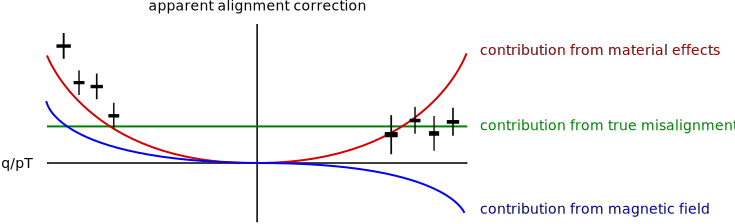
\includegraphics[width=\linewidth]{removing_magnetic_field.png}

\label{numpages}
\end{frame}

\end{document}
